\documentclass[conference]{IEEEtran}
\usepackage[utf8]{inputenc}
\IEEEoverridecommandlockouts
% The preceding line is only needed to identify funding in the first footnote. If that is unneeded, please comment it out.
%Template version as of 6/27/2024

\usepackage{cite}


\usepackage{amsmath,amssymb,amsfonts}
\usepackage{algorithmic}
\usepackage{graphicx}
\usepackage{textcomp}
\usepackage{xcolor}
\usepackage{hyperref}
\usepackage{physics}
\usepackage{float}
\usepackage{inputenc}

% Add TikZ package and necessary libraries
\usepackage{tikz}
\usetikzlibrary{arrows.meta,positioning,fit,backgrounds,shapes.geometric}

% Add circuitikz package for circuit diagrams
\usepackage{circuitikz}

% Add float control parameters to help with figure placement
\renewcommand{\floatpagefraction}{0.8}
\renewcommand{\topfraction}{0.8}
\renewcommand{\bottomfraction}{0.8}
\renewcommand{\textfraction}{0.1}
\setcounter{totalnumber}{50}
\setcounter{topnumber}{50}
\setcounter{bottomnumber}{50}

% Force LaTeX to place figures earlier
\renewcommand{\dblfloatpagefraction}{0.7}
\renewcommand{\dbltopfraction}{0.8}

\def\BibTeX{{\rm B\kern-.05em{\sc i\kern-.025em b}\kern-.08em
    T\kern-.1667em\lower.7ex\hbox{E}\kern-.125emX}}
\begin{document}

\title{Medical Imaging Classification with Cold-Atom Reservoir Computing using Auto-Encoders and Surrogate-Driven Training\\
% {\footnotesize \textsuperscript{*}Note: Sub-titles are not captured for https://ieeexplore.ieee.org  and
% should not be used}
}

\author{\IEEEauthorblockN{Anonymous Authors}}
% \author{
% \IEEEauthorblockN{Nuno Batista}
% \IEEEauthorblockA{\textit{Department of Informatics Engineering} \\
% \textit{Faculty of Sciences and Technology, University of Coimbra}\\
% Coimbra, Portugal \\
% \href{mailto:nunomarquesbatista@gmail.com}{nunomarquesbatista@gmail.com}}

% \and
% \IEEEauthorblockN{2\textsuperscript{nd} Given Name Surname}
% \IEEEauthorblockA{\textit{dept. name of organization (of Aff.)} \\
% \textit{name of organization (of Aff.)}\\
% City, Country \\
% email address or ORCID}
% }

\maketitle

%ADD SPACE TO BREATHE

\begin{abstract}
We introduce a quantum-classical hybrid 
architecture for medical image classification 
based on neutral atom quantum processors. 
This approach is designed to address the challenges of 
medical imaging, with a particular focus on tasks such 
as polyp detection and classification.
By integrating an autoencoder guided by a quantum 
reservoir, the pipeline learns compact and discriminative 
representations of image data that are also well-suited for quantum reservoir 
computing. To overcome the non-differentiability of quantum 
measurements, we circumvent this `gradient barrier' 
by incorporating a differentiable surrogate model that simulates the 
behaviour of the quantum layer, enabling end-to-end backpropagation. 
The guided training process jointly optimizes for both image 
reconstruction and classification accuracy, ensuring that the latent 
representations are both meaningful and effective for quantum processing. 
In our implementation, image data is encoded as atom detuning parameters 
in a Rydberg Hamiltonian, and quantum embeddings are obtained through expectation 
values. These embeddings are then passed to a linear classifier, 
enabling faster training and inference compared to deep classical networks.
Our experiments show that this method outperforms traditional 
approaches using PCA or unguided autoencoders. We also conduct 
ablation studies to evaluate the impact of quantum and training 
parameters, demonstrating the robustness and flexibility of the 
proposed pipeline for real-world medical imaging applications, 
even in the NISQ era.
\end{abstract}

\begin{IEEEkeywords}
Reservoir Computing, Quantum-Guided Autoencoding,
Neutral Atoms, Autoencoder, Dimensionality Reduction, 
Quantum Machine Learning, Hybrid Quantum-Classical Algorithms, 
Medical Image Classification, Quantum Surrogate Models
\end{IEEEkeywords}

%============================================
% INTRODUCTION
%============================================
\section{Introduction}

\subsection{Background and Motivation}
Advances in medical imaging have significantly improved 
disease diagnosis and treatment planning. For conditions 
like colorectal cancer, early detection of polyps through 
colonoscopy image analysis is critical for reducing mortality~\cite{estevaGuideDeepLearning2019}. 
Deep learning techniques, especially autoencoders, are widely 
used to extract compressed, informative features from 
high-dimensional images for classification and segmentation 
tasks~\cite{bengioLearningDeepArchitectures}. However, classical neural networks may struggle 
to capture intricate correlations in complex medical data.

Quantum computing offers novel opportunities 
for machine learning, particularly through quantum reservoir 
computing (QRC), where a physical quantum system processes 
classical inputs into high-dimensional nonlinear embeddings~\cite{tanakaRecentAdvancesPhysical2019,fujiiHarnessingDisorderedQuantum2017}. Recent works show that analog quantum systems, 
such as neutral-atom platforms, can serve as untrained 
reservoirs with rich dynamics for temporal and pattern 
recognition tasks \cite{domingoOptimalQuantumReservoir2022,kornjavcaLargescaleQuantumReservoir2024}. 
In hybrid approaches, a classical encoder compresses 
image data, and a quantum reservoir expands 
the encoded features into a higher-dimensional space, 
potentially boosting classification performance.

A major challenge in such hybrid quantum-classical 
models is the non-differentiability of quantum measurements, 
which obstructs gradient-based optimization. Additionally, 
tuning quantum parameters can suffer from barren plateaus, where 
gradients vanish in high-dimensional Hilbert spaces \cite{mccleanBarrenPlateausQuantum2018}. 
To address this, we introduce a classical neural surrogate 
that emulates the quantum reservoir's input-output behavior. 
This surrogate enables end-to-end training via backpropagation, 
while the quantum system remains fixed and non-trainable.


\subsection{Contributions of This Work}
We propose a quantum-guided autoencoder architecture that 
integrates a classical image encoder with a neutral-atom
quantum reservoir.

A classical surrogate network of the reservoir itself enables 
gradient flow through the whole model during training.

Our results illustrate the viability of QRC for real-world medical 
tasks and offer a scalable path to hybrid quantum-classical learning,
even in the noisy intermediate-scale quantum (NISQ) era.


%============================================
% BACKGROUND 
%============================================
\section{Background and Related Work}

\subsection{Principles of Reservoir Computing}
Reservoir computing is a computational framework 
derived from recurrent neural networks (RNNs). It 
involves a fixed, high-dimensional dynamical system—the 
reservoir—that projects input data into a rich feature 
space. Only the output layer is trained, simplifying 
the learning process and reducing computational 
overhead. This approach is particularly effective 
for time-series prediction and pattern recognition tasks.

Mathematically, let \( u(t) \in \mathbb{R}^m \) be the input at time \( t \),
\( x(t) \in \mathbb{R}^n \) the reservoir state, and
\( y(t) \in \mathbb{R}^k \) the output. The reservoir dynamics
and output are given by:
\begin{equation}
    x(t) = f(W_{in} u(t) + W_{res} x(t-1))
\end{equation}
\begin{equation}
    y(t) = W_{out} x(t)
\end{equation}

%Where ff is a nonlinear activation function, WinWin​ and WW are fixed input and reservoir weight matrices, and WoutWout​ is the trained output weight matrix.

Where \( f \) is a nonlinear activation function,
\( W_{in} \) and \( W_{res} \) are fixed input and reservoir weight matrices, 
and \( W_{out} \) is the trained output weight matrix.

A diagram of a typical Reservoir Computing architecture is shown in `Fig.-\ref{fig:reservoir_architecture}'.

\begin{figure}[!h]
    \centering
    \resizebox{\columnwidth}{!}{%
        \begin{circuitikz}
            \tikzstyle{every node}=[font=\normalsize]
            \draw(6,-1.5) circle (0.25cm);
            \draw(6,-2.25) circle (0.25cm);
            \draw(6,-3) circle (0.25cm);
            \draw(6,-0.75) circle (0.25cm);
            \draw(7.5,-1) circle (0.25cm);
            \draw(8,-1.5) circle (0.25cm);
            \draw(8.25,-2.25) circle (0.25cm);
            \draw(7.75,-2.75) circle (0.25cm);
            \draw(8.5,-0.5) circle (0.25cm);
            \draw(9.25,-2.25) circle (0.25cm);
            \draw(9.75,-0.5) circle (0.25cm);
            \draw(9.25,-1.25) circle (0.25cm);
            \draw(9.75,-3) circle (0.25cm);
            \draw(8.75,-3.25) circle (0.25cm);
            \draw(10.5,-2.25) circle (0.25cm);
            \draw(10.5,-1.25) circle (0.25cm);
            \draw[->, >=Stealth] (8,-2.75) .. controls (8,-3.25) and (8.25,-3.25) .. (8.5,-3.25) ;
            \draw[->, >=Stealth] (8,-2.75) .. controls (8.75,-3) and (8.5,-2.25) .. (9,-2.25) ;
            \draw[->, >=Stealth] (9,-3.25) .. controls (9.25,-3.5) and (9.5,-3.25) .. (9.5,-3) ;
            \draw[->, >=Stealth] (10,-3) .. controls (10.75,-3.5) and (10.5,-2.75) .. (10.5,-2.5) ;
            \draw[->, >=Stealth] (9.5,-2.25) -- (10.25,-1.25);
            \draw[->, >=Stealth] (10.25,-2.25) -- (9.5,-1.25);
            \draw[->, >=Stealth] (8.5,-2.25) .. controls (9,-1.75) and (8.75,-1.75) .. (9,-1.25) ;
            \draw[->, >=Stealth] (9.25,-1) .. controls (9,-1) and (9.25,-0.5) .. (8.75,-0.5) ;
            \draw[->, >=Stealth] (7.75,-1) .. controls (7.75,-0.75) and (7.75,-0.5) .. (8.25,-0.5) ;
            \draw[->, >=Stealth] (8.25,-1.5) .. controls (8.75,-1.25) and (8.5,-1) .. (8.5,-0.75) ;
            \draw[->, >=Stealth] (9.5,-0.5) .. controls (9.5,0) and (9.25,0) .. (8.75,-0.5) ;
            \draw(12,-1) circle (0.25cm);
            \draw(12,-1.75) circle (0.25cm);
            \draw(12,-2.5) circle (0.25cm);
            \draw[->, >=Stealth] (10,-0.5) -- (11.75,-1);
            \draw[->, >=Stealth] (10.75,-1.25) -- (11.75,-1.75);
            \draw[->, >=Stealth] (10.75,-2.25) -- (11.75,-2.5);
            \draw[ dashed] (5.5,0.25) rectangle  (6.5,-4);
            \draw[ dashed] (7,0.25) rectangle  (11,-4);
            \draw[ dashed] (11.5,0.25) rectangle  (12.5,-4);
            \draw[->, >=Stealth] (6.25,-0.75) -- (7.25,-1);
            \draw[->, >=Stealth] (6.25,-1.5) -- (7.75,-1.5);
            \draw[->, >=Stealth] (6.25,-2.25) -- (8,-2.25);
            \draw[->, >=Stealth] (6.25,-3) -- (7.5,-2.75);
            \node[font=\normalsize] at (6,0.5) {Input Layer};
            \node[font=\normalsize] at (9,0.5) {Reservoir Layer};
            \node[font=\normalsize] at (12,0.5) {Output Layer};
            \node[font=\normalsize] at (5,-2) {$u(t)$};
            \node[font=\normalsize] at (10.5,-3.5) {$W_{res}$};
            \node[font=\normalsize] at (13,-2) {$y(t)$};
            \node[font=\normalsize] at (6.8,-4.3) {$W_\text{in}$};
            \node[font=\normalsize] at (10.5,-0.2) {$x(t)$};
            \node[font=\normalsize] at (11.2,-4.3) {$W_\text{out}$};
        \end{circuitikz}
    }%

\caption{
    Reservoir computing architecture showing input nodes, 
    a recurrent reservoir network with internal dynamics, 
    and an output layer.
}
\label{fig:reservoir_architecture}
\end{figure}


\subsection{Quantum Reservoir Computing}
Quantum Reservoir Computing (QRC) extends the reservoir 
computing paradigm into the quantum domain. By leveraging quantum systems' 
inherent properties, such as superposition and entanglement, QRC aims 
to enhance computational capabilities. Implementations using quantum 
oscillators have shown promise in solving complex learning tasks, 
offering advantages over classical counterparts. Notably, large-scale 
experiments utilizing neutral-atom analog quantum computers have demonstrated 
the scalability and effectiveness of QRC in various machine learning applications~\cite{kornjavcaLargescaleQuantumReservoir2024}


In QRC, classical input data \( u(t) \) is encoded into quantum states \( |\psi(t)\rangle \),
which evolve under a fixed Hamiltonian \( H \):
\begin{equation}
    |\psi(t+1)\rangle = U |\psi(t)\rangle = e^{-iH\Delta t} |\psi(t)\rangle,
\end{equation}
where \( U \) is the unitary evolution operator. Measurements of observables \( \hat{O} \) yield outputs:
\begin{equation}
    y(t) = \langle \psi(t) | \hat{O} | \psi(t) \rangle.
\end{equation}
The output weights are trained classically, while the quantum reservoir remains fixed.

\subsection{Reservoir Computing with Neutral Atoms}
As Quantum Reservoir Computing (QRC) leverages the complex 
dynamics of quantum systems to process information, 
extending the Classical Reservoir Computing 
paradigm into the quantum domain. Neutral atom platforms, 
particularly those utilizing Rydberg states, 
have emerged as promising candidates for implementing 
QRC due to their scalability and controllable interactions.

In the work by M. Kornjača et al.~\cite{kornjavcaLargescaleQuantumReservoir2024}, 
a large-scale, gradient-free QRC algorithm was 
developed and experimentally implemented on a 
neutral-atom analog quantum computer. 
This system achieved competitive performance across 
various machine learning tasks, 
including classification and time-series prediction, 
demonstrating effective learning with increasing system 
sizes up to 108 qubits.

The dynamics of such neutral atom systems can be 
described by the Rydberg Hamiltonian, which captures 
the essential physics of laser-driven interactions 
among atoms in Rydberg states. Following Kornjača et al.~\cite{kornjavcaLargescaleQuantumReservoir2024}
the Hamiltonian for a system of neutral-atoms is given by:

\begin{equation}
    \begin{aligned}
        H(t) &= \dfrac{\Omega(t)}{2}\sum_j \left(\ket{g_j}\bra{r_j}+\ket{r_j}\bra{g_j}\right) \\
             &{{\quad}} + \sum_{j<k}V_{jk}n_jn_k - \sum_j \left[\Delta_{\mathrm{g}}(t) + \alpha_j\Delta_{\mathrm{l}}(t)\right] n_j,
    \end{aligned}
    \label{eq:rydberg_hamiltonian}
\end{equation}
where \( \Omega(t) \) is the global Rabi drive amplitude between a 
ground state \( |g_j\rangle \) and a highly-excited Rydberg state 
\( |r_j\rangle \) of an atom,
\( n_j = |r_j\rangle \langle r_j| \), 
\( V_{jk} = C/\|r_j - r_k\|^6 \) describes the van der Waals interactions
between atoms, and the detuning is split into a global term 
\( \Delta_{\mathrm{g}}(t) \)
and a site-dependent term \( \Delta_{\mathrm{l}}(t) \), with site 
modulation \( \alpha_j \in [0, 1] \).

By initializing the system in a specific state and allowing 
it to evolve under this Hamiltonian, the resulting quantum 
state encodes information about the input data. Measurements 
of observables on this state yield outputs that can be used 
for tasks such as classification or prediction, with only the 
final readout layer requiring training.


\subsection{Dimensionality Reduction for Image Data}
Dimensionality reduction is a crucial preprocessing step in 
machine learning and data analysis, aiming to reduce the 
number of input variables in a dataset while preserving as 
much information as possible. This process enhances 
computational efficiency, mitigates the curse of 
dimensionality, and facilitates data visualization


\subsubsection{Principal Component Analysis}
Principal Component Analysis (PCA)~\cite{shlensTutorialPrincipalComponent2014} is a linear dimensionality 
reduction technique that transforms a set of correlated 
variables into a set of uncorrelated variables called 
principal components. The goal is to capture the maximum 
variance in the data with the fewest number of components.

PCA is effective for datasets where the principal components 
align with the directions of maximum variance, but it may not 
capture complex, nonlinear relationships in the data~\cite{jolliffePrincipalComponentAnalysis2016}.

\subsubsection{Autoencoder Architectures}
Autoencoders are a class of artificial neural networks 
designed to learn efficient codings of input data in an 
unsupervised manner. They consist of two main parts: an 
encoder that compresses the input into a latent-space 
representation, and a decoder that reconstructs the input 
from this representation.

Given an input \( x \in \mathbb{R}^d \), the encoder maps 
\( x \) to a latent representation \( z \in \mathbb{R}^k \) 
(where \( k < d \)):

\begin{equation}
    z = f_\theta(x)
\end{equation}

The decoder then reconstructs the input:
\begin{equation}
    \hat{x} = g_\phi(z)
\end{equation}
The network is trained to minimize the reconstruction loss:
\begin{equation}
    \mathcal{L}(x, \hat{x}) = \| x - \hat{x} \|^2
\end{equation}

This typical architecture of an autoencoder is illustrated in 
`Fig.-\ref{fig:autoencoder_architecture}'.

\begin{figure}[!t]
    \centering
    \resizebox{\columnwidth}{!}{%
        \begin{circuitikz}
            \tikzstyle{every node}=[font=\LARGE]
            \draw[ fill={rgb,255:red,246; green,245; blue,244} ] (4.25,11.75) rectangle (5.5,10.5);
            \draw[ fill={rgb,255:red,246; green,245; blue,244} ] (4.75,11.25) rectangle (6,10);
            \node[font=\LARGE] at (5,12.25) {x};
            \draw[->, >=Stealth] (6,11) -- (8,11);
            \draw(8,12.25) rectangle  node {\Huge $f_{\theta}(x)$} (10.5,9.75);
            \node[font=\large] at (9.5,11.25) {};
            \node[font=\large] at (9,10.5) {};
            \node[font=\large] at (10.5,11.25) {};
            \draw[short] (13.75,11.5) -- (10.5,12.25);
            \draw[short] (10.5,9.75) -- (13.75,10.5);
            \draw(13.75,11.75) rectangle  node {\LARGE z} (14.5,10);
            \draw(17.75,12.25) rectangle  node {\Huge $g_{\phi}(z)$} (20.25,9.75);
            \draw[short] (17.75,12.25) -- (14.5,11.5);
            \draw[short] (14.5,10.5) -- (17.75,9.75);
            \node[font=\Large] at (14,13.75) {Autoencoder};
            \node[font=\large] at (10,12.75) {Encoder Network};
            \node[font=\large] at (18.25,12.75) {Decoder Network};
            \draw[->, >=Stealth] (20.25,11) -- (22.25,11);
            \draw[ fill={rgb,255:red,154; green,153; blue,150} ] (22.75,11.75) rectangle (24,10.5);
            \draw[ fill={rgb,255:red,154; green,153; blue,150} ] (22.25,11.25) rectangle (23.5,10);
            \node[font=\LARGE] at (23,12.25) {$\hat{x}$};
            \draw[<->, >=Stealth, dashed] (5.25,11.75) .. controls (7.5,16.25) and (21.75,15.75) .. (23,11.75)node[pos=0.5, fill=white]{$\mathcal{L}$};
            \node[font=\huge] at (17.75,51.5) {};
            \node[font=\Large] at (14,12.25) {Latent};
        \end{circuitikz}
    }%
    
\caption{
    Autoencoder architecture. The encoder network $f_{\theta}(x)$ 
    compresses the input $x$ into a latent representation $z$, while the decoder 
    network $g_{\phi}(z)$ reconstructs the input from the latent representation, 
    producing $\hat{x}$. The reconstruction loss $\mathcal{L}$ measures the 
    compresses the input $x$ into a latent representation $z$, while the decoder 
    network $g_{\phi}(z)$ reconstructs the input from the latent representation, 
    producing $\hat{x}$.
}
\label{fig:autoencoder_architecture}
\end{figure}


Autoencoders can capture complex, nonlinear 
relationships in the data, making them suitable for tasks 
like image compression, denoising, and anomaly 
detection~\cite{hintonReducingDimensionalityData2006, estevaGuideDeepLearning2019}.

\subsubsection{Quantum-Guided Autoencoding}
Quantum-Guided Autoencoders integrate quantum 
computing principles into the autoencoder framework 
to leverage quantum advantages in processing and 
representing data. These models aim to perform 
dimensionality reduction and classification within a 
single architecture, enhancing performance on complex 
datasets.

In the Quantum-Guided Autoencoder (QGAE) model, a 
classical encoder first reduced the dimensionality
of the input data. The compressed data is then processed 
by a parametrized quantum circuit, which acts as the decoder
and classifier. The quantum circuit transforms the 
input state \( |\psi_{\text{in}}\rangle \) into an
output state \( |\psi_{\text{out}}\rangle \) using a unitary operation
\begin{equation}
    |\psi_{\text{out}}\rangle = U(\theta) |\psi_{\text{in}}\rangle
\end{equation}
Measurements on \( |\psi_{\text{out}}\rangle \) yield the final
classification result. The parameters \( \theta \) are
optimized to minimize a loss function that combines
reconstruction error and classification accuracy.


This approach has demonstrated improved performance 
over traditional methods in tasks such as identifying 
the Higgs boson in particle collision data, 
showcasing the potential of quantum-guided models in 
handling high-dimensional, complex datasets~\cite{belisGuidedQuantumCompression2024}.

%============================================
% METHODOLOGY
%============================================
\section{Methodology}
\subsection{System Architecture Overview}

Our proposed pipeline integrates classical and quantum 
components for dimensionality reduction and classification. 
A classical autoencoder compresses high-dimensional image 
data into a lower-dimensional latent space. This latent 
representation is encoded into a Rydberg atom chain, 
serving as input to a quantum reservoir. The reservoir's 
dynamics, governed by the Rydberg Hamiltonian, produce 
quantum embeddings through measurements of quantum observables.
The overall architecture is illustrated in `Fig.-\ref{fig:qgars_pipeline}'.

To facilitate end-to-end training, we employ a differentiable 
surrogate model that approximates the quantum reservoir's 
behavior, enabling gradient flow from the classification 
loss back to the autoencoder. The surrogate's outputs feed 
into a linear classifier trained to map quantum embeddings to class labels.

The autoencoder is trained to minimize a combined loss 
function that interpolates between reconstruction loss and 
classification loss, promoting representations that are both 
informative for input reconstruction and effective for quantum 
reservoir computing.

Once trained, the encoder compresses data into the latent 
space, which is then processed by the actual quantum reservoir. 
The resulting quantum embeddings are used to train a linear 
classifier for final predictions.


\begin{figure*}[!h]
    \centering
    \resizebox{0.9\textwidth}{!}{
        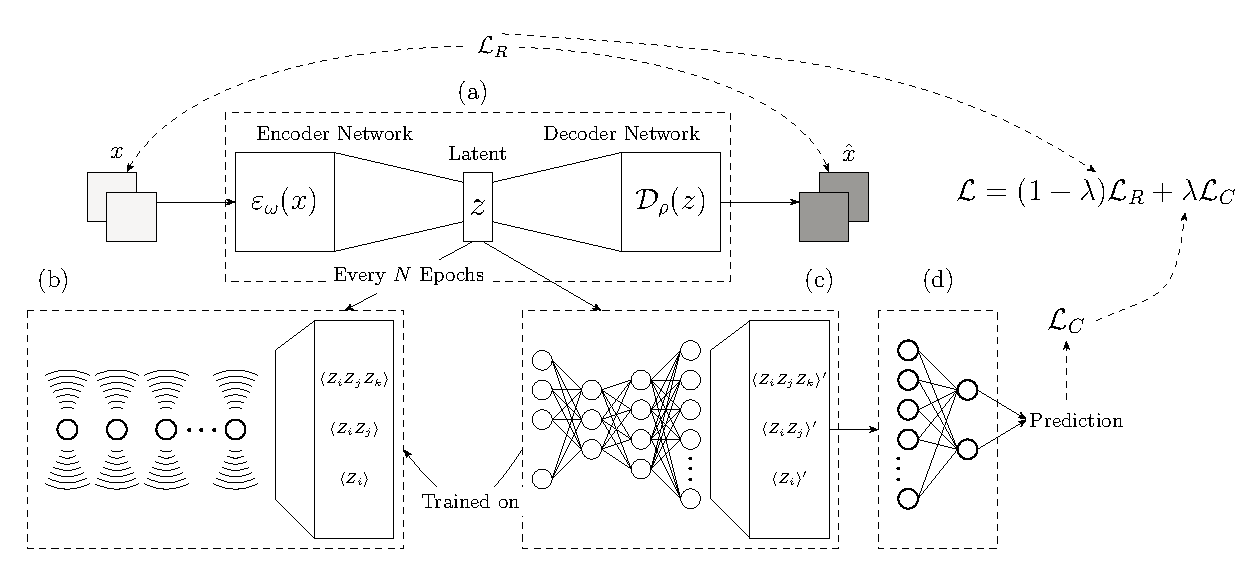
\includegraphics{qgars_pipeline_cropped.pdf}
    }
    \label{fig:qgars_pipeline}
    \caption{Overview of the Quantum-Guided Autoencoder Reservoir Computing System.}
\end{figure*}

\subsection{Quantum Guided Autoencoder}
The Quantum Guided Autoencoder (QGA) combines classical 
preprocessing with quantum processing to leverage 
the strengths of both paradigms. The classical encoder 
reduces the dimensionality of the input data, facilitating 
efficient quantum processing. The quantum circuit 
then processes the compressed data, aiming to reconstruct 
the original input and perform classification simultaneously.

\subsubsection{Loss Function Design}
The QGA is trained to minimize a composite loss 
function that balances reconstruction fidelity and 
classification accuracy:

\begin{equation}
    \mathcal{L} = (1-\lambda) \cdot \mathcal{L}_R + \lambda \cdot \mathcal{L}_{C},
    \label{eq:composed_loss_function}
\end{equation}
where:
\begin{itemize}
    \item \( \mathcal{L}_R = \| x - \hat{x} \|^2 \) is the reconstruction loss, measuring the mean squared error between the input \( x \) and its reconstruction \( \hat{x} \).
    \item \( \mathcal{L}_C = -\sum_i y_i \log(\hat{y}_i) \) is the classification loss, computed as the cross-entropy between the true labels \( y_i \) and the predicted probabilities \( \hat{y}_i \).
    \item \( 0 < \lambda < 1 \) is a hyperparameter that controls the trade-off between reconstruction and classification objectives.
\end{itemize}    

%\subsubsection{Balancing Reconstruction and Classification}


\subsection{The Gradient Barrier Problem}
Hybrid quantum-classical models, such as the Quantum Guided Autoencoder 
(QGAE), aim to leverage quantum computational advantages within 
classical machine learning frameworks. However, a significant 
challenge arises due to the non-differentiable nature of quantum 
operations, commonly referred to as the `gradient barrier'.

In classical neural networks, training relies on backpropagation, 
which requires the computation of gradients through all components 
of the network. In hybrid models, the inclusion of quantum 
layers introduces operations that are inherently non-differentiable:

\begin{itemize}
    \item \textbf{Quantum State Preparation}: 
    Encoding classical data into 
    quantum states often involves operations 
    that are not smoothly differentiable with 
    respect to the input data.
    
    \item \textbf{Quantum Measurements}:
    Observing quantum states collapses them, 
    introducing stochasticity and breaking the 
    deterministic gradient flow required 
    for backpropagation.
\end{itemize}

These aspects hinder the direct application of 
gradient-based optimization methods across the 
quantum-classical boundary, obstructing end-to-end 
training of hybrid models. The surrogate model 
solution, proposed in the next section, addresses 
this problem.

\subsection{Surrogate Modeling for Quantum Layers}
To circumvent the gradient barrier, surrogate models 
have been proposed. These are classical, differentiable 
models trained to approximate the input-output behavior 
of quantum circuits. By replacing the non-differentiable 
quantum components with their surrogate counterparts during 
training, gradients can be propagated through the entire network, 
enabling end-to-end optimization. 

Recent studies have demonstrated the efficacy of 
surrogate models in mitigating the effects of barren plateaus 
and facilitating the training of hybrid quantum-classical models. 
These approaches allow for the practical implementation of 
quantum-enhanced machine learning models by leveraging classical 
optimization techniques while still capturing quantum computational 
advantages~\cite{xieQuantumSurrogateDrivenImage2025b}


\subsubsection{Architecture}
In our pipeline, the surrogate model is implemented as a 
feedforward neural network designed to learn the mapping 
from the autoencoder's latent space to the quantum 
embeddings produced by the quantum reservoir. 

Its architecture comprises multiple fully connected 
layers with nonlinear activation functions, facilitating 
the approximation of the complex, non-linear 
transformations inherent in quantum dynamics.

This approach draws inspiration from recent studies 
demonstrating the effectiveness of surrogate models 
in approximating quantum circuit behaviors, thereby 
facilitating efficient training of hybrid 
models.~\cite{xieQuantumSurrogateDrivenImage2025b,schreiberClassicalSurrogatesQuantum2023}

\subsubsection{Training Procedure}
\begin{itemize}
    \item Data Input: 
    Feed a batch of latent data \( z \) from the autoencoder 
    into the real quantum reservoir, recording the resulting quantum 
    embeddings.

    \item Surrogate Training:
    Train the surrogate model using the recorded quantum
    embeddings as targets, minimizing the loss function:
    \begin{equation}
        \mathcal{L}_{\text{surrogate}} = \| \hat{y} - y \|^2,
    \end{equation}
    where \( \hat{y} \) are the surrogate model's predictions
    and \( y \) are the actual quantum embeddings.

    \item Regular Updates:
    Periodically update the surrogate model during training
    to insure it accurately reflects the quantum reservoir's
    behavior. This can be done after a fixed number of epochs
    or when the surrogate's performance on a validation set
    reaches a certain threshold.
\end{itemize}

\subsubsection{Gradient Flow Through Surrogate Models}
By integrating the surrogate model into the training pipeline, 
we establish a continuous computational graph from the 
output layer back to the input layer, enabling the use of 
gradient-based optimization techniques. The surrogate model 
serves as a differentiable proxy for the quantum reservoir, 
allowing the classification loss to influence the 
autoencoder's parameters effectively.

As a results, we not only achieve end-to-end training of the
hybrid model but also makes it computationally efficient,
as we reduce the need for frequent quantum measurements.

\subsection{Rydberg Hamiltonian and Quantum Dynamics}
The quantum reservoir in our architecture is implemented
using a neutral-atom system, specifically utilizing
Rydberg atoms to create a programmable quantum reservoir.
The dynamics of the system are governed by the Rydberg Hamiltonian,
which describes the interactions between atoms in Rydberg states~\ref{eq:rydberg_hamiltonian}.

\subsubsection{Data Encoding Schemes}
The input data is encoded into the quantum system by mapping
the latent representations from the autoencoder to the
detuning parameters of the Rydberg Hamiltonian.
This encoding process involves adjusting the detuning
parameters \( \Delta_{\mathrm{l}}(t) \) for each atom in the chain,
allowing the system to represent the input data in a way that
is compatible with the quantum dynamics of the reservoir.

\subsubsection{Quantum Readout Methods}
The quantum reservoir's output is obtained by probing, 
in successive time steps, the state of the atoms 
after the systems evolution up to a certain time \( t \).

The readout is performed by measuring specific observables,
such as $\langle Z_i \rangle$, $\langle Z_i \, Z_j\rangle$, and $\langle Z_i \, Z_j \, Z_k \rangle$, which measure respectively one-, two- and three-qubit correlations.
% \begin{itemize}
%     \item \textbf{Single-atom Measurements}: 
%     \( \langle Z_i \rangle \) for each atom \( i \), where \( Z_i \) is the Pauli-Z operator.
%     \item \textbf{Two-atom Correlations}: 
%     \( \langle Z_i Z_j \rangle \) for pairs of atoms \( (i, j) \), capturing correlations between their states.
%     \item \textbf{Three-atom Correlations}:
%     \( \langle Z_i Z_j Z_k \rangle \) for triplets of atoms \( (i, j, k) \), providing higher-order correlations.
% \end{itemize}

%============================================
% EXPERIMENTAL SETUP
%============================================
\section{Experimental Setup}
\subsection{Datasets}
We evaluate our proposed architecture on three primary datasets:
\begin{enumerate}
    \item \textbf{Synthetic Polyp Dataset:} 
    A synthetic dataset of polyp images generated to simulate 
    realistic medical imaging scenarios.
    
    \item \textbf{CVC-ClinicDB Dataset:} 
    Real image patches extracted from the CVC-ClinicDB 
    dataset, a well-known benchmark for polyp detection. 
    This dataset provides a diverse set of polyp images 
    with varying characteristics, allowing for robust 
    evaluation of classification performance.
    
    \item \textbf{MNIST Dataset:} 
    A reduced version of the MNIST dataset, 
    containing only the digits 0 and 1, suitable 
    for binary classification tasks. This dataset 
    serves as a controlled environment to assess 
    the model's performance on simpler classification tasks.
\end{enumerate}

\subsection{Feature Reduction Methods}
We implemented and compared three distinct feature reduction approaches:
\subsubsection{Principal Component Analysis (PCA)}
PCA was employed as a baseline linear 
dimensionality reduction technique. 
We extracted the top-k principal components 
(typically 4-12) from the flattened image data, 
which were then used as inputs to both classical and 
quantum-enhanced classifiers.

\subsubsection{Autoencoder}
We implemented a neural network-based autoencoder with the following architecture:

\begin{itemize}
    \item An encoder network that compresses
    the input to a lower-dimensional latent space.
    
    \item A decoder network that reconstructs 
    the original input from the latent representation

    \item Batch normalization and dropout layers 
    to improve training stability and prevent overfitting.
\end{itemize}

The autoencoder was trained to minimize reconstruction 
loss using the Adam optimizer with learning rates 
between $0.001$--$0.01$ and weight decay for regularization.

\subsubsection{Quantum-Guided Autoencoder}
We introduced a quantum-guided autoencoder 
that incorporates feedback from the quantum 
reservoir during training. This approach combines:

\begin{itemize}
    \item A standard autoencoder architecture
    \item A linear classifier that maps quantum embeddings to class labels.
    \item A classification loss computed on quantum embeddings
    \item A weighting parameter $\lambda$ to control the trade-off between 
    reconstruction and classification objectives~\ref{eq:composed_loss_function}.
    \item A differentiable surrogate model that approximates the quantum reservoir's behavior,
    enabling end-to-end backpropagation through the entire pipeline. The frequency 
    of quantum updates is controlled by a hyperparameter, allowing for
    flexible integration of quantum dynamics into the training process.
\end{itemize}


\subsubsection{Quantum Reservoir Computing Layer}
Our quantum reservoir computing implementation uses 
a Rydberg atom simulator with the following parameterizable
components:

\begin{itemize}
    \item \textbf{Atom Chain Length:} 
    The number of atoms in the chain, which can be adjusted 
    to control the reservoir's capacity and complexity.
    
    \item \textbf{Rabi Frequency:} 
    The global Rabi drive amplitude, which influences the 
    strength of interactions between atoms.
    
    \item \textbf{Detuning Parameters:} 
    Site-dependent detuning parameters that encode the input data.
    
    \item \textbf{Measurement Strategy:} 
    The specific observables measured to obtain quantum embeddings.

    \item \textbf{Encoding Scale:}
    The scale of the input data encoding, which can be adjusted
    to optimize the quantum reservoir's response to the input data.

    \item \textbf{Time steps:}
    The number of time steps for which the quantum reservoir evolves,
    allowing for the capture of temporal dynamics in the data.
\end{itemize}

\subsubsection{Classical Network Architectures}
After the traning process of the quantum-guided autoencoder,
the following quantum embeddings are passed to a linear classifier.
The classifier is a simple feedforward neural network with the following architecture:
\begin{itemize}
    \item A single hidden layer with a ReLU activation function.
    \item Cross-entropy loss for training, optimized using the Adam optimizer.
\end{itemize}

\subsection{Comparison Methods}
We benchmarked our model against some
classical methods, including:
\begin{itemize}
    \item \textbf{PCA + Linear Classifier:} 
    A linear classifier trained on the PCA-reduced features.
    
    \item \textbf{Autoencoder + Linear Classifier:} 
    A linear classifier trained on the latent representations from the autoencoder.
    
    \item \textbf{PCA + Neural Network:}
    A fully connected neural network trained on the PCA-reduced features.
    
    \item \textbf{Autoencoder + Neural Network:}
    A fully connected neural network trained on the latent representations from the autoencoder.
\end{itemize}

\subsection{Performance Metrics}
We evaluated the performance of our model using the following metrics:
Classification Accuracy, F1 Score, Confusion Matrix.

% \begin{itemize}
%     \item \textbf{Classification Accuracy} 
%     %The percentage of correctly classified instances in the test set.
    
%     \item \textbf{F1 Score} 
%     %The harmonic mean of precision and recall, providing a balanced measure of %classification performance.
    
%     \item \textbf{Confusion Matrix} 
%    % A matrix summarizing the classification results, showing true positives, %false positives, true negatives, and false negatives.
    
% \end{itemize}


\subsection{Parameter Sweep Strategy}
To optimize the performance of our quantum-guided autoencoder, 
we conducted a systematic parameter sweep over the following hyperparameters:
\begin{itemize}
    \item \textbf{Guided Lambda Parameter (\( \lambda \))}: 
    This parameter controls the trade-off between reconstruction and classification objectives in the loss function~\ref{eq:composed_loss_function}. We tested values ranging from 0.1 to 0.9 in increments of 0.1.

    \item \textbf{Quantum Update Frequency:} 
    The frequency at which the quantum reservoir is updated during training. We experimented with update frequencies of 1, 5, and 10 epochs.

    \item \textbf{Quantum Parameters:} 
    Including the number of atoms in the chain, Rabi frequency, and detuning parameters. We varied these parameters to assess their impact on classification performance.
    \item \textbf{Batch Size:}
    \item \textbf{Learning Rate:}
\end{itemize}

%============================================
% RESULTS
%============================================
\section{Results and Discussion}
\subsection{Classification Performance Comparison}
\subsection{Ablation Studies}
\subsubsection{Impact of Guided Lambda Parameter}
\subsubsection{Effect of Quantum Update Frequency}
\subsubsection{Influence of Quantum Parameters}
\subsection{Dimensionality Reduction Comparison}
\subsection{Surrogate Model Fidelity Analysis}
\subsection{Generalization to Unseen Data}


%============================================
% LIMITATIONS AND FUTURE WORK
%============================================
\section{Limitations and Future Work}
\subsection{Current Limitations}
\subsection{Potential Extensions}
\subsection{Hardware Implementation Considerations}

%============================================
% CONCLUSION
%============================================
\section{Conclusion}

%============================================
% REFERENCES
%============================================
\bibliographystyle{IEEEtran}
\bibliography{references}

\newpage
\newpage
\tableofcontents

\end{document}